%%%%%%%%%%%%%%%%%%%%%%%%%%%%%%%%%%%%%%%%%%%%%%%%%%%%%%%%%%%%%%%%%%%%%%%%%%%%%%%%
\documentclass[presentation]{beamer} %\mode<presentation>{\usetheme{sapere}}
\usetheme{CambridgeUS}
\usecolortheme{orchid}

\definecolor{themeColor}{HTML}{11AD1E}

\setbeamercolor*{structure}{bg=black,fg=themeColor}

\setbeamercolor*{palette primary}{use=structure,fg=white,bg=structure.fg}
\setbeamercolor*{palette secondary}{use=structure,fg=white,bg=structure.fg!75}
\setbeamercolor*{palette tertiary}{use=structure,fg=white,bg=structure.fg!50!black}
\setbeamercolor*{palette quaternary}{fg=white,bg=black}

\setbeamercolor{section in toc}{fg=black,bg=white}
\setbeamercolor{alerted text}{use=structure,fg=structure.fg!50!black!80!black}

\setbeamercolor{titlelike}{parent=palette primary,fg=structure.fg!50!black}
\setbeamercolor{frametitle}{bg=structure.fg!10!white,fg=structure.fg!50!black!80!black}

\setbeamercolor*{titlelike}{parent=palette primary}

\usepackage[utf8]{inputenc}
\usepackage{amssymb}
\usepackage{graphicx}
\usepackage{subfigure}
\usepackage{multirow}
\usepackage{hhline}
\usepackage{amsfonts,amstext,amssymb,wasysym}
\usepackage{fancyvrb}
\usepackage{alltt}
\usepackage{textcomp}
\usepackage{url}
\usepackage{multimedia,pgf}
\usepackage{geometry}
\usepackage{listings}
\usepackage{framed}
\usepackage{cleveref}

% Names
\newcommand{\alchemist}{{\sf ALCHEMIST}}

\title[Computational Fields and Augmented Reality]{Computational Fields meet Augmented Reality: Perspectives and Challenges}

\author[Pianini et. al]{
Danilo Pianini, Angelo Croatti, Mirko Viroli, Alessandro Ricci\\
\texttt{{\footnotesize \{danilo.pianini, a.croatti, mirko.viroli, a.ricci\}@unibo.it}}}


\institute[UniBo]
{\textsc{Alma Mater Studiorum}---Universit\`a di Bologna a Cesena}

\date[2015-09-21 SCOPES]{Spatial and COllective PErvasive Computing Systems (SCOPES)\\
\scriptsize September 21, 2015 - Cambridge, USA
}

\pgfdeclareimage[height=0.625cm]{university-logo}{imgs/logo}
\logo{\pgfuseimage{university-logo}}


\begin{document}


%===============================================================================
\frame[label=coverpage]{\titlepage}
%===============================================================================

\section*{Outline}
%===============================================================================
\frame{\tableofcontents}

%===============================================================================
\section{Introduction}
%===============================================================================

\subsection{Motivation}
\begin{frame}{Why Augmented Reality (AR) and Computational Fields (CF)?}
  \begin{block}{Differences}
    They are definitely different entities
    \begin{itemize}
      \item CF is a programming abstraction. AR is a mean of interaction.
      \item CF focuses on collectivity, AR (mostly) on the single user.
    \end{itemize}
  \end{block}
  \begin{block}{Commonalities}
    They share a common context of application
    \begin{itemize}
      \item Both are devoted at environments pervaded with computational devices
      \item Both are bound to the physical world
    \end{itemize}
  \end{block}
\end{frame}


%===============================================================================
\section{Augmented Reality}
%===============================================================================
\begin{frame}{Definition}
  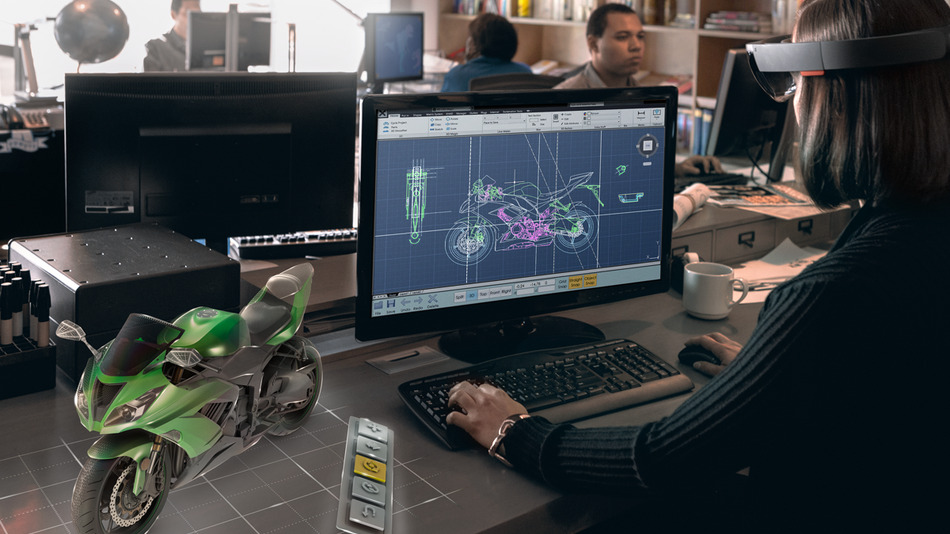
\includegraphics[width=.49\textwidth]{images/holobike}
  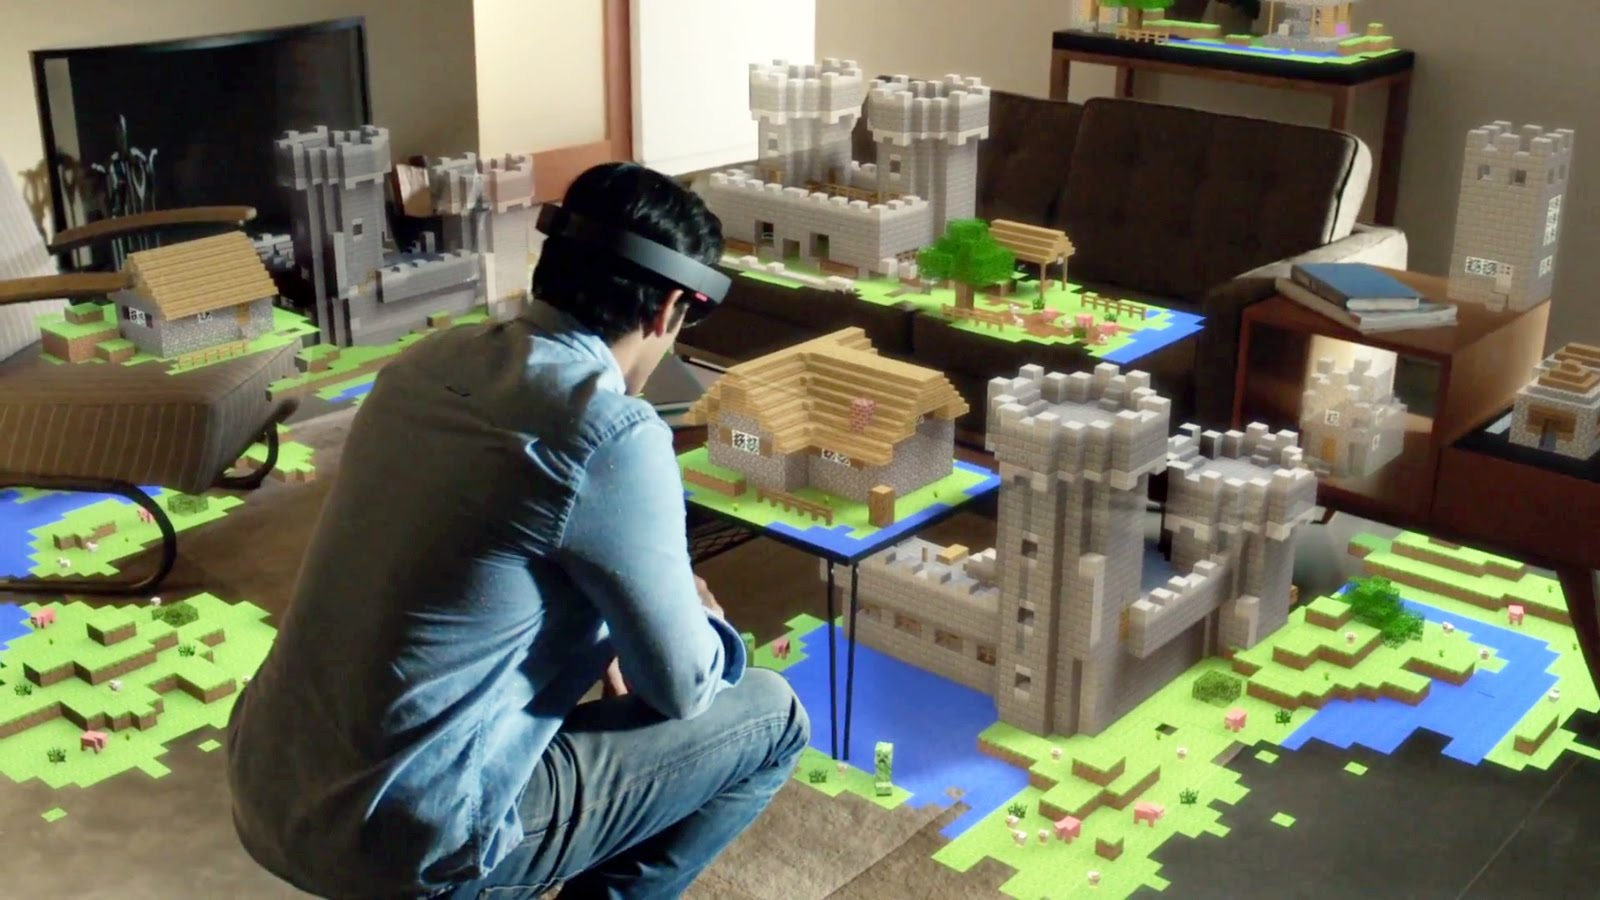
\includegraphics[width=.49\textwidth]{images/holominecraft}
  \begin{block}{Augmented Reality}
    is a technology that allows the user to see the \textbf{real world, with virtual objects} superimposed upon or mixed with the real world \cite{Azuma97}.
    \begin{itemize}
      \item The ultimate goal is a seamless integration of reality and virtuality
      \item Mostly via see-through devices
    \end{itemize}
  \end{block}
  \begin{center}
    \tiny{Images from Microsoft Hololens presentation video}
  \end{center}
\end{frame}

\begin{frame}{Degrees of augmentation}
  Augmentation can happen at different levels:
  \begin{enumerate}
    \item \textbf{Unrelated} to the elements in the user's FOV
      \begin{itemize}
        \item E.g. displaying a map on a visual overlay
      \end{itemize}
    \item \textbf{Dynamically associated} to elements in the user's FOV
      \begin{itemize}
        \item E.g. displaying historical information next to a monument in FOV
      \end{itemize}
    \item \textbf{Entirely virtual and interactive} elements on real world
      \begin{itemize}
        \item E.g. the two images of the previous slide, the ghost game \cite{MirrorWorlds}
      \end{itemize}
  \end{enumerate}
\end{frame}

%===============================================================================
\section{Computational fields}
%===============================================================================
%-------------------------------------------------------------------------------
\subsection{The concept of field}
%-------------------------------------------------------------------------------
%-------------------------------------------------------------------------------
\subsection{Protelis: a language for aggregate computing}
%-------------------------------------------------------------------------------
citare ieee computer
%===============================================================================
\section{Augmented Fields}
%===============================================================================
%-------------------------------------------------------------------------------
\subsection{Augmented reality as visual interface for fields}
%-------------------------------------------------------------------------------
%-------------------------------------------------------------------------------
\subsection{Augmented reality-based input for CF program}
%-------------------------------------------------------------------------------
%-------------------------------------------------------------------------------
\subsection{Computational fields as enabling technology for AR applications}
%-------------------------------------------------------------------------------
%-------------------------------------------------------------------------------
\subsection{Examples}
%-------------------------------------------------------------------------------
%===============================================================================
\section{Conclusion}
%===============================================================================



\section*{\refname}
%===============================================================================
\begin{frame}[allowframebreaks]
%\begin{frame}[t,allowframebreaks]
  \frametitle{\refname}
  \scriptsize
  \bibliographystyle{alpha}
  \bibliography{bibliography}
\end{frame}
\section*{\refname}




\end{document}